\documentclass[12pt,a4paper]{article}

%%%%%%%%%%%%%%%%%%%%%%%%%%%%%%%%%%%%%%%%%%%%%%%%%%%%%%%%%%%%%%%%%%%%%
%    DOCUMENT TITLE

\newcommand{\doctitle}{Titolo}

%%%%%%%%%%%%%%%%%%%%%%%%%%%%%%%%%%%%%%%%%%%%%%%%%%%%%%%%%%%%%%%%%%%%%
%%%%%%%%%%%%%%%%%%%%%%%%%%%%%%%%%%%%%%%%%%%%%%%%%%%%%%%%%%%%%%%%%%%%%
%%%%%%%%%%%%%%%%%%%%%%%%%%%%%%%%%%%%%%%%%%%%%%%%%%%%%%%%%%%%%%%%%%%%%
%   DOCUMENT SUBTITILE

\newcommand{\docsubtitle}{Sottotitolo}

%%%%%%%%%%%%%%%%%%%%%%%%%%%%%%%%%%%%%%%%%%%%%%%%%%%%%%%%%%%%%%%%%%%%%
%%%%%%%%%%%%%%%%%%%%%%%%%%%%%%%%%%%%%%%%%%%%%%%%%%%%%%%%%%%%%%%%%%%%%
%%%%%%%%%%%%%%%%%%%%%%%%%%%%%%%%%%%%%%%%%%%%%%%%%%%%%%%%%%%%%%%%%%%%%
%   DOCUMENT FOOTER 
%  
% If not modified, footer is equal to document subtitle

\newcommand{\projectfooter}{\docsubtitle}

%%%%%%%%%%%%%%%%%%%%%%%%%%%%%%%%%%%%%%%%%%%%%%%%%%%%%%%%%%%%%%%%%%%%%
%%%%%%%%%%%%%%%%%%%%%%%%%%%%%%%%%%%%%%%%%%%%%%%%%%%%%%%%%%%%%%%%%%%%%
%%%%%%%%%%%%%%%%%%%%%%%%%%%%%%%%%%%%%%%%%%%%%%%%%%%%%%%%%%%%%%%%%%%%%
%    AUTHOR(S)
%  
% Verisioning Table

\newcommand{\printVersioning}{
	\centering
	\begin{tabular}{l l}

		\textbf{Data} & \textbf{Autore della modifica} \\ 
		\hline 
		&  \\ 
		\hline 
	\end{tabular} 
}

%%%%%%%%%%%%%%%%%%%%%%%%%%%%%%%%%%%%%%%%%%%%%%%%%%%%%%%%%%%%%%%%%%%%%
%%%%%%%%%%%%%%%%%%%%%%%%%%%%%%%%%%%%%%%%%%%%%%%%%%%%%%%%%%%%%%%%%%%%%
%%%%%%%%%%%%%%%%%%%%%%%%%%%%%%%%%%%%%%%%%%%%%%%%%%%%%%%%%%%%%%%%%%%%%
\usepackage{tikz}
\usepackage{tikz-uml}
\usepackage{graphicx}    
\usepackage{float}
\usepackage{hyperref}                   % collegamenti ipertestuali
\usepackage[utf8]{inputenc}
\usepackage[italian]{babel}
\usepackage[babel]{csquotes}
\usepackage{url}
\usepackage{graphicx}
\usepackage{lastpage}
\usepackage{fancyhdr}
\usepackage[top=1cm,bottom=4cm,left=80pt,right=80pt]{geometry} %disegna la linea
\usepackage{listings} %per grandi porzioni di codice
\usepackage{booktabs,tabularx}
\usepackage{makeidx}
\usepackage{fixltx2e}
\usepackage{hyperref}
\usepackage{enumitem}
\usepackage{color}
\usepackage[T1]{fontenc}
\usepackage{svg}
\usepackage{amsmath}
\usepackage[toc]{glossaries}
\usepackage{dirtree}
\usepackage{listings}
\usepackage{siunitx}
\usepackage[official]{eurosym}
\usepackage[export]{adjustbox}
\usepackage{calc}
\usepackage{rotating}
\usepackage{soul}
\usepackage{amsmath}

\pagestyle{fancy}
\setlength{\headheight}{2cm} %settato grandezza header

\renewcommand{\footrulewidth}{0.5pt} %ridefinisco il valore della riga di intestazione
\renewcommand{\headrulewidth}{0.5pt} %ridefinisco il valore della riga di pie' di pagina
\addtolength{\headwidth}{\marginparsep}
\addtolength{\headwidth}{\marginparwidth}

\fancyhead{} %annulla head di default
\fancyfoot{} %annulla foot di default

\newcommand{\pkg}{\section }
\newcommand{\class}{\subsection}
\newcommand{\pkgclass}[2]{\subsection{{#2}.{#1}}}
\newcommand{\mainpkgclass}[2]{\subsection{{#2}.{#1}}}
\newcommand{\oneclass}[2]{\paragraph{{#2}.{#1}}}

\newcommand{\oo}[1]{\subitem[out]\texttt{ #1}}
\newcommand{\ov}{\subitem[out]\texttt{ void}}
\newcommand{\ob}{\subitem[out]\texttt{ bool}}
\newcommand{\ii}[1]{\subitem[in]\texttt{ #1}}
\newcommand{\ib}[1]{\subitem[in]\texttt{#1:bool}}
\newcommand{\mh}[1]{\item\texttt{ #1}}
\newcommand{\true}{\texttt{true}}
\newcommand{\false}{\texttt{false}}
\newcommand{\complex}[1]{\textit{\color{blue} {#1}}}
\newcommand{\change}[1]{\textit{ \color{red}** {#1}}}

\usepackage{listings}
\usepackage[most]{tcolorbox}
\usepackage{inconsolata}



\newtcblisting[auto counter]{codebox}[2][]{sharp corners, 
	fonttitle=\bfseries, colframe=gray, listing only, 
	listing options={basicstyle=\ttfamily,language=java}, 
	}

%	Logo intestazione
\rhead{\includegraphics[scale=0.15]{ITRspinoff.png}}

%	footer
\cfoot{
	\projectfooter\\
	{\doctitle}\\
%	{\tiny Questo documento è distribuito sotto licenza {..}}
}
\rfoot{
	\thepage\ di \pageref{LastPage}
}


%**************************************************************
% Impostazioni di hyperref
%**************************************************************
\hypersetup{
	%hyperfootnotes=false,
	%pdfpagelabels,
	%draft,	% = elimina tutti i link (utile per stampe in bianco e nero)
	colorlinks=true,
	linktocpage=true,
	pdfstartpage=1,
	pdfstartview=FitV,
	% decommenta la riga seguente per avere link in nero (per esempio per la stampa in bianco e nero)
	%colorlinks=false, linktocpage=false, pdfborder={0 0 0}, pdfstartpage=1, pdfstartview=FitV,
	breaklinks=true,
	pdfpagemode=UseNone,
	pageanchor=true,
	pdfpagemode=UseOutlines,
	plainpages=false,
	bookmarksnumbered,
	bookmarksopen=true,
	bookmarksopenlevel=1,
	hypertexnames=true,
	pdfhighlight=/O
}
\newcommand{\printTitle}{	
	\begin{titlepage}
		\begin{center}
			
			\begin{figure}[h!]	\vspace{5cm}
				\centering
				\includegraphics[width=0.7\linewidth]{ITRspinoff}
			\end{figure}
			\vspace{0.3cm}
			\hrule
			\vspace{0.3cm}	
			\begin{Huge}
				\doctitle  \\			
			\end{Huge}
			\vspace{0.3cm}
			\begin{Large}
				\docsubtitle
			\end{Large}
			\vspace{0.3cm}
			
		\end{center}
		
\end{titlepage}}





	\begin{document}
	\printTitle
	\newpage
	\tableofcontents
	\newpage
	%\listoftables
	%\listoffigures
	Metodi e Modelli per l’Ottimizzazione Combinatoria
	Progetto d’esame, aa 2017-2018
	Anna Bonaldo
  \section{	Modellazione }
	Il problema da affrontare può essere rappresentato in modo generico come un insieme di punti in uno spazio bidimensionale. In particolare, è modellabile come un TSP asimmetrico, in quanto è sufficiente utilizzare spigoli (e non archi orientati) per rappresentare il percorso eseguito per la foratura di una scheda. La direzione in cui viene eseguito il percorso non è influente sul tempo impiegato per percorrere l’intero tragitto. 
	
	Le istanze del problema su cui vengono testati gli algoritmi (esatti ed euristici) sono di più tipologie: 
	\begin{itemize}
	\item	Punti generati randomicamente in uno spazio di raggio determinato. Questo insieme di istanze del problema rappresenta un caso molto generico, e compare spesso anche in letteratura, per svariate tipologie di analisi sugli algoritmi per la risoluzione del TSP. In particolare, vengono utilizzate più misure per il raggio in cui generare casualmente i punti. In seguito una tabella che elenca tutte le possibilità esaminate.

	
	\subitem    Dataset RANDN	raggio uguale alla dimensione del problema. 
	\subitem 	CONSTRAND50	Raggio costante uguale a 50	
	\subitem 	CONSTRAND5000 Raggio costante uguale a 5000
	\subitem 	GRI	N punti disposti a griglia di lato $\sqrt{N}$ equi distanziati. 
	\\
	\begin{center}


	\begin{tabular}{lllll}
		
		N punti	&  RANDN 
		 &	CONSTRAND50
	 &	CONSTRAND5000
			& GRID \\
		
   \hline 
	10 punti &	Raggio 10 &	Raggio 50&	Raggio 5000 &	Griglia di 10 punti\\

	50 punti &	Raggio 50&	Raggio 50&	Raggio 5000&	Griglia di 50 punti\\
 
	100 punti&	Raggio 100&	Raggio 50&	Raggio 5000&	Griglia di 100 punti\\

	200 punti &	Raggio 200&	Raggio 50&	Raggio 5000	&Griglia di 200 punti\\	
	\hline 
\end{tabular} 
	\end{center}

	\item Punti posizionati “a griglia”, tra loro uniformemente distanziati. Questo insieme di istanze del problema, invece, è probabilmente più aderente al problema in questione. E’ infatti probabile che nel caso in esame i punti in cui eseguire la foratura non siano sparsi casualmente sulla superficie dell’oggetto. 
	\end{itemize}
	
	Le varie tipologie di dataset utilizzati sono state scelte per confrontare gli effetti della morfologia del problema sulle prestazioni dell’algoritmo utilizzato per la risoluzione. 
	\subsection{Struttura del progetto}
	
	Il progetto include: 
	\begin{itemize}


	\item	Una prima parte realizzata con l’utilizzo del framework \textbf{CPlex Studio}, utilizzata per la risoluzione delle istanze di TSP con metodi esatti. 
	\item	Una seconda parte, realizzata in \textbf{c++, in ambiente Windows 10 }(Visual Studio 2017) per la risoluzione delle istanze del TSP con metodi euristici. Il programma realizzato utilizza la libreria OpenCV per rappresentare graficamente (e salvare su file) le soluzioni calcolate delle istanze del problema. 
		\end{itemize}
	
	\section{Implementazione dei metodi euristici per la soluzione del TSP}
	I metodi euristici implementati sono i seguenti: 
	\begin{itemize}
	\item	\textbf{Greedy Nearest-Neighbour}
	Ad ogni passo di esecuzione sceglie come nuovo passo del cammino il punto più vicino tra quelli disponibili. Viene mantenuta una lista sei nodi non ancora inclusi nel cammino.
	L’insieme dei nodi “liberi”, ovvero non inclusi nel cammino, è implementata attraverso la struttura datdella libreria standard c++. Quest’ultima permette di verificare in tempo $O(\log n)$ se un nodo è già stato inserito nel cammino. 
	Poiché ad ogni passo è necessario scegliere il nodo a distanza minima tra i disponibili, questa implementazione ha un tempo di esecuzione che è al più $O(n! \log(n))$. E’ possibile realizzare implementazioni, un po’ più complesse ma più efficienti, utilizzando strutture dati più complesse. 

	\item \textbf{Simulated Annealing}
\item \textbf{Tabu Search}

\end{itemize}
	
\subsubsection{	Ottimizzazione delle soluzioni esistenti}
	Algoritmo di ottimizzazione di un percorso basato su euristica 2-opt
	L’implementazione verifica per ogni coppia di archi nel cammino corrente se tali archi sono tra loro secati. In se la soluzione ottenuta eliminando l’incrocio tra due archi nel percorso è migliore della corrente, la nuova soluzione prende il posto di quella attuale. Poiché l’algoritmo deve iterare su tutte le coppie di archi, la complessità del calcolo è di O(n2) .  I test per verificare se due archi sono secanti occupano un tempo O(1), utilizzando semplici nozioni geometriche per verificare la presenza di intersezioni. 
\section{Dataset}
	
	Tutti i dataset utilizzati sono stati prodotti utilizzando Cplex Studio. \\
	Questi, una volta generati, vengono salvati su file e riutilizzati da tutti gli algoritmi implementati. In questo modo si assicura che i risultati possano essere tra loro confrontabili. 
	
	Per quanto riguarda il dataset GRID, lo script realizzato produce una sola istanza del problema per ogni dimensione considerata(10, 50, 100 e 200 punti). Questa scelta è motivata dal fatto che la procedura di realizzazione di una griglia è deterministica. 
	
	Per quanto riguarda i restanti dataset: \textbf{RAND N }, \textbf{CONSTRAND50}, e \textbf{CONSTRAND5000} vengono \textbf{prodotte 10 diverse istanze del problema} per ogni dimensione considerata. Ogni generazione di un’istanza per un certo dataset utilizza un diverso seed, per inizializzare la funzione rand().In questo modo si ha una discreta rappresentazione della variabilità del problema per il dataset considerato.
\section{Analisi dei dati}

\subsection{Soluzione esatta del TSP}	
	L’implementazione dell’algoritmo esatto del TSP realizzata con CPLEX Studio è stata utilizzata per risolvere il problema su tutti i dataset utilizzati. Le soluzioni ottenute sono state poi utilizzare come punto di riferimento per valutare gli algoritmi euristici.

	I\textbf{ tempi medi} per il calcolo della soluzione con metodi esatti sono riportati in tabella 
    TODO, con la relativa deviazione standard. 

	Dai risultati si evince che la densità di punti generati nello spazio bidimensionale non influenza la varianza del tempo di calcolo. Al contrario se con il numero di punti del problema  diminuisce anche la relativa densità nello spazio (e quindi aumenta il raggio entro cui vengono generati i punti del problema), la deviazione standard aumenta in modo considerevole. Se ne deriva che l’algoritmo utilizzato ha più difficlotà nel trovare la soluzione. 
	Per quanto riguarda il problema con 200 punti, il programma fallisce con errore per insufficienza di memoria disponibile. Non si dispone quindi di una soluzione esatta. Per i successivi calcoli che vengono valutati in rapporto alla soluzione esatta, si utilizza in sostituzione della soluzione ottima (non disponibile) la migliore soluzione ottenuta con algoritmi euristici.  

	Il tempo di calcolo per ottenere la soluzione esatta è notoriamente esponenziale sulla dimensione del problema. Il grafico riporta i dati medi per ogni dataset. Si evidenzia che il raggio entro cui sono distribuiti i punti del problema influenza in modo negativo i tempi di calcolo della soluzione. In particolar modo, il caso in cui il raggio dello spazio dei punti sia ugiale ad N (numero di punti) appare particolarmente critico.
	
	\subsection{TSP Greedy Nearest Neighbors}
	L’euristica costruttiva Nearest Neighbours  rappresenta un metodo molto veloce per il calcolo della soluzione del TSP. Tuttavia la qualità della soluzione non è generalmente buona nel caso generico. Per quanto riguarda casi particolari, come ad esempio per il dataset GRID, in cui i punti sono disposti regolarmente, si riescono ad ottenere soluzioni buone anche con il solo utilizzo di questa euristica. Si veda un esempio in figura. TODO 
	
	E' tuttavia possibile migliorare i risultati ottenuti utilizzando un'euristica \textit{2-Opt} che elimina eventuali spigoli che si intersecano nel cammino calcolato. 
	Nell'esperimento realizzato, si vede che l'utilizzo di un'ottimizzazione \textit{2-opt} su una soluzione  precalcolata con Greedy Nearest Neighbours porta a buone soluzioni in tempi inferiori ad euristiche come Tabu Search e Simulated Annealing \ref{fig:greedyoptimprove}. 

	\begin{figure}[h!]
		\centering
		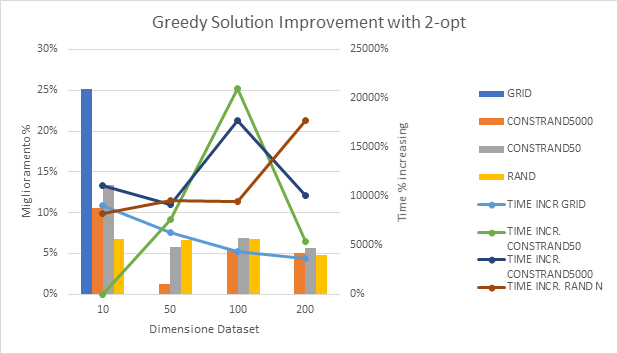
\includegraphics[width=0.7\linewidth]{img/GreedyOptImprove}
		\caption{}
		\label{fig:greedyoptimprove}
	\end{figure}
     
     Con questo metodo, per i dataset utilizzati, in generale, si ottengono soluzioni migliori in media del 5\% rispetto alla soluzione con solo algoritmo Greedy per problemi di dimensione maggiore o uguale a 50 nodi. Per problemi di dimensione inferiore, il guadagno in termine di bontà della soluzione è tra il 5 ed il 15\%. 
     
     Essendo la procedura di ottimizzazione \textit{2-Opt} $O(n^{2}) $, il tempo di calcolo in rapporto al precedente aumenta in modo considerevole (fino al 20000\%). Tuttavia rimane inferiore a quello necessario ad altri algoritmi (Simluated Annealing) per produrre soluzioni peggiori. TODO
     
	 \subsection{Simulated Annealing}
	 \begin{figure}[h!]
	 	\centering
	 	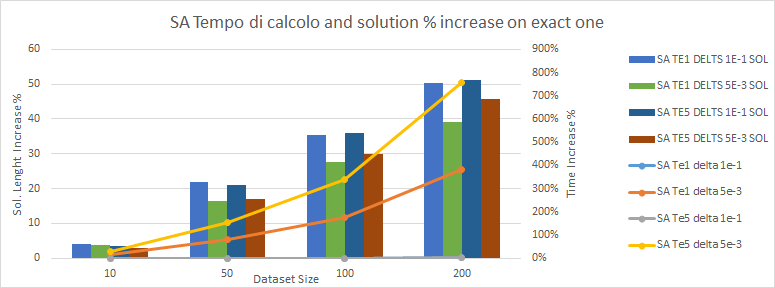
\includegraphics[width=0.7\linewidth]{img/SASolAndTimeIncrease}
	 	\caption{}
	 	\label{fig:sasolandtimeincrease}
	 \end{figure}
	 
	 \subsection{Tabu Search} 
	
	\section{Compilazione del progetto}
	
	\appendix
	
\end{document}